% Source PDF page 259 (printed p. 245)
求解这组含 $m+n$ 个方程、$m+n$ 个变量 $x^\star,\nu^\star$ 的方程组，即可得到（5.50）的最优原始和对偶变量。
\end{origexample}

\begin{origexample}{5.2}
\emph{注水。}考虑凸优化问题
\[
\begin{array}{ll}\text{最小化}&-\sum_{i=1}^n\log(\alpha_i+x_i)\\
\text{约束为}&x\succeq0,\quad\one^\T x=1,\end{array}
\]
其中 $\alpha_i>0$。这一问题出现在信息论中，用于向 $n$ 个通信信道分配功率。变量 $x_i$ 是分配给第 $i$ 个信道的发射功率，$\log(\alpha_i+x_i)$ 给出信道容量或通信速率，因此问题是将总量为1的功率分配给各信道，使总通信速率最大。

对不等式约束 $x^\star\succeq0$ 引入拉格朗日乘子 $\lambda^\star\in\R^n$，对等式约束 $\one^\T x=1$ 引入乘子 $\nu^\star\in\R$，得到KKT条件
\[
\begin{gathered}
x^\star\succeq0,\quad\one^\T x^\star=1,\quad\lambda^\star\succeq0,\quad
\lambda_i^\star x_i^\star=0,\quad i=1,\ldots,n,\\
-1/(\alpha_i+x_i^\star)-\lambda_i^\star+\nu^\star=0,\quad i=1,\ldots,n.
\end{gathered}
\]
可以直接求解这些方程，得到 $x^\star,\lambda^\star,\nu^\star$。首先注意，$\lambda^\star$ 在最后一个方程中起松弛变量的作用，可将其消去，得到
\[
\begin{gathered}
x^\star\succeq0,\quad \one^\T x^\star=1,\quad
x_i^\star\bigl(\nu^\star-1/(\alpha_i+x_i^\star)\bigr)=0,\quad i=1,\ldots,n,\\
\nu^\star\ge1/(\alpha_i+x_i^\star),\quad i=1,\ldots,n.
\end{gathered}
\]
若 $\nu^\star<1/\alpha_i$，最后一个条件只有在 $x_i^\star>0$ 时才可能成立；再由第三个条件，得到 $\nu^\star=1/(\alpha_i+x_i^\star)$。解出 $x_i^\star$，可知当 $\nu^\star<1/\alpha_i$ 时，$x_i^\star=1/\nu^\star-\alpha_i$。若 $\nu^\star\ge1/\alpha_i$，则不可能有 $x_i^\star>0$，否则将有 $\nu^\star\ge1/\alpha_i>1/(\alpha_i+x_i^\star)$，违反互补松弛。因此，当 $\nu^\star\ge1/\alpha_i$ 时，$x_i^\star=0$。所以
\[
x_i^\star=\begin{cases}
1/\nu^\star-\alpha_i&\nu^\star<1/\alpha_i,\\
0&\nu^\star\ge1/\alpha_i,
\end{cases}
\]
更简洁地，$x_i^\star=\max\{0,1/\nu^\star-\alpha_i\}$。代入 $\one^\T x^\star=1$，得到
\[
\sum_{i=1}^n\max\{0,1/\nu^\star-\alpha_i\}=1.
\]
左端是关于 $1/\nu^\star$ 的分段线性递增函数，折点为 $\alpha_i$，因此方程有容易求出的唯一解。

这种求解方法称为\emph{注水}，原因如下。将 $\alpha_i$ 看作第 $i$ 块地面的高度，然后向区域注水，水位为 $1/\nu$，如图5.7所示。总用水量为 $\sum_{i=1}^n\max\{0,1/\nu^\star-\alpha_i\}$。逐渐提高水位，直到总用水量恰为1。此时第 $i$ 块地面上方的水深就是最优值 $x_i^\star$。
\end{origexample}

% Source PDF page 260 (printed p. 246)
\begin{figure}[htbp]\centering
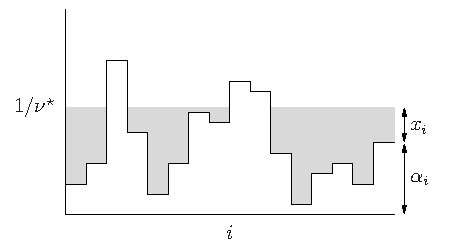
\includegraphics[width=.65\linewidth]{figures/ch05-fig07.pdf}
\caption*{图5.7\quad 注水算法示意图。各块地面的高度为 $\alpha_i$。将区域注水到水位 $1/\nu^\star$，总用水量为1。各块地面上方的水深（阴影部分）就是 $x_i^\star$ 的最优值。}
\end{figure}
\begin{figure}[htbp]\centering
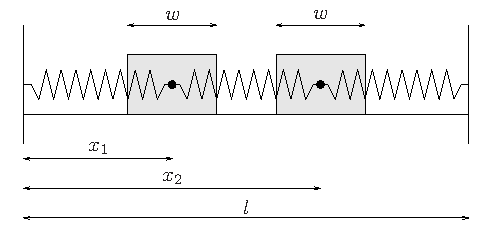
\includegraphics[width=.65\linewidth]{figures/ch05-fig08.pdf}
\caption*{图5.8\quad 两个物块由弹簧相互连接，并与左右墙壁连接。物块宽度为 $w>0$，不能相互穿透，也不能穿过墙壁。}
\end{figure}

\subsection{KKT条件的力学解释}
KKT条件在力学中有一个很好的解释（这事实上也是Lagrange的主要动机之一）。用一个简单例子来说明。图5.8中的系统由两个物块组成，三个弹簧将它们相互连接，并连接到左右墙壁。物块位置由 $x\in\R^2$ 给出，$x_1$ 是左侧物块（中心）的位移，$x_2$ 是右侧物块的位移。左墙位置为0，右墙位置为 $l$。

弹簧势能是物块位置的函数：
\[
f_0(x_1,x_2)=\frac12k_1x_1^2+\frac12k_2(x_2-x_1)^2+\frac12k_3(l-x_2)^2,
\]
其中 $k_i>0$ 为三个弹簧的刚度系数。平衡位置 $x^\star$ 是在以下不等式约束下使势能最小的位置：
\begin{equation}
w/2-x_1\le0,\qquad w+x_1-x_2\le0,\qquad w/2-l+x_2\le0.\tag{5.51}
\end{equation}

% Source PDF page 261 (printed p. 247)
\begin{figure}[htbp]\centering
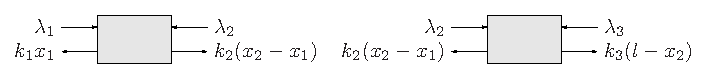
\includegraphics[width=.85\linewidth]{figures/ch05-fig09.pdf}
\caption*{图5.9\quad 物块—弹簧系统的受力分析。弹簧力和接触力作用在每个物块上的合力必须为零。上方所示拉格朗日乘子是墙壁与物块之间的接触力，下方表示弹簧力。}
\end{figure}
这些约束称为\emph{运动学约束}，表达物块宽度为 $w>0$、不能相互穿透或穿过墙壁这一事实。因此，平衡位置由下列二次规划的解给出：
\begin{equation}
\begin{array}{ll}
\text{最小化}&(1/2)\bigl(k_1x_1^2+k_2(x_2-x_1)^2+k_3(l-x_2)^2\bigr)\\
\text{约束为}&w/2-x_1\le0\\
&w+x_1-x_2\le0\\
&w/2-l+x_2\le0.
\end{array}\tag{5.52}
\end{equation}
取 $\lambda_1,\lambda_2,\lambda_3$ 为拉格朗日乘子，该问题的KKT条件由运动学约束（5.51）、非负约束 $\lambda_i\ge0$、互补松弛条件
\begin{equation}
\begin{gathered}
\lambda_1(w/2-x_1)=0,\quad
\lambda_2(w-x_2+x_1)=0,\\
\lambda_3(w/2-l+x_2)=0,
\end{gathered}\tag{5.53}
\end{equation}
以及零梯度条件
\begin{equation}
\begin{bmatrix}k_1x_1-k_2(x_2-x_1)\\k_2(x_2-x_1)-k_3(l-x_2)\end{bmatrix}
+\lambda_1\begin{bmatrix}-1\\0\end{bmatrix}
+\lambda_2\begin{bmatrix}1\\-1\end{bmatrix}
+\lambda_3\begin{bmatrix}0\\1\end{bmatrix}=0\tag{5.54}
\end{equation}
组成。

如果把拉格朗日乘子解释为墙壁与物块之间的接触力，方程（5.54）就可理解为两个物块的力平衡方程，如图5.9所示。第一个方程表示第一个物块上的合力为零：$-k_1x_1$ 是左弹簧对左物块的作用力，$k_2(x_2-x_1)$ 是中间弹簧的作用力，$\lambda_1$ 是左墙的作用力，$-\lambda_2$ 是右物块的作用力。接触力必须指向离开接触面的方向（由 $\lambda_1\ge0$、$-\lambda_2\le0$ 表达），并且只有发生接触时才非零（由前两个互补松弛条件（5.53）表达）。类似地，（5.54）的第二个方程是第二个物块的力平衡方程；（5.53）的最后一个条件表示，除非右物块碰到墙壁，否则 $\lambda_3$ 为零。

这个例子中，势能和运动学约束函数均凸，而且只要 $2w\le l$，即两墙之间有足够空间容纳两个物块，就满足Slater约束资格的放宽形式。因此可知，由（5.52）给出的平衡能量表述，与KKT条件给出的力平衡表述产生相同结果。

% Source PDF page 262 (printed p. 248)
\subsection{通过对偶求解原始问题}
在§5.5.3开头已提到，若强对偶成立且对偶最优解 $(\lambda^\star,\nu^\star)$ 存在，那么任意原始最优点也是 $L(x,\lambda^\star,\nu^\star)$ 的最小点。有时可利用这一事实，从对偶最优解计算原始最优解。

更准确地说，假设有强对偶且已知最优的 $(\lambda^\star,\nu^\star)$。再假设 $L(x,\lambda^\star,\nu^\star)$ 的最小点，即问题
\begin{equation}
\text{最小化}\quad f_0(x)+\sum_{i=1}^m\lambda_i^\star f_i(x)
+\sum_{i=1}^p\nu_i^\star h_i(x)\tag{5.55}
\end{equation}
的解是唯一的。（对于凸问题，例如当 $L(x,\lambda^\star,\nu^\star)$ 关于 $x$ 严格凸时，就会如此。）若（5.55）的解原始可行，则它必定原始最优；若它原始不可行，则原始最优点不可能存在，即可知原始最优值不能达到。当对偶问题比原始问题容易求解时，例如对偶可以解析求解，或具有可利用的特殊结构时，这一观察很有意义。

\begin{origexample}{5.3}
\emph{熵最大化。}考虑熵最大化问题
\[
\begin{array}{ll}\text{最小化}&f_0(x)=\sum_{i=1}^n x_i\log x_i\\
\text{约束为}&Ax\preceq b\\&\one^\T x=1,\end{array}
\]
定义域为 $\R_{++}^n$。它的对偶为
\[
\begin{array}{ll}\text{最大化}&-b^\T\lambda-\nu-e^{-\nu-1}\sum_{i=1}^n e^{-a_i^\T\lambda}\\
\text{约束为}&\lambda\succeq0,\end{array}
\]
其中 $a_i$ 是 $A$ 的各列（见第222、228页）。假设较弱的Slater条件成立，即存在 $x\succ0$ 满足 $Ax\preceq b$、$\one^\T x=1$。因此强对偶成立，且最优解 $(\lambda^\star,\nu^\star)$ 存在。

设已求出对偶问题的解。在 $(\lambda^\star,\nu^\star)$ 处的拉格朗日函数为
\[
L(x,\lambda^\star,\nu^\star)=\sum_{i=1}^n x_i\log x_i
+(\lambda^\star)^\T(Ax-b)+\nu^\star(\one^\T x-1).
\]
它在 $D$ 上严格凸且有下界，所以有唯一解 $x^\star$，由下式给出：
\[
x_i^\star=1/\exp(a_i^\T\lambda^\star+\nu^\star+1),\quad i=1,\ldots,n.
\]
若 $x^\star$ 原始可行，则必为原始问题（5.13）的最优解；若 $x^\star$ 原始不可行，则可知原始最优值不能达到。
\end{origexample}

\begin{origexample}{5.4}
\emph{等式约束下可分函数的最小化。}考虑问题
\[
\begin{array}{ll}\text{最小化}&f_0(x)=\sum_{i=1}^n f_i(x_i)\\
\text{约束为}&a^\T x=b,\end{array}
\]

% Source PDF page 263 (printed p. 249)
其中 $a\in\R^n$、$b\in\R$，$f_i:\R\to\R$ 可微且严格凸。目标函数称为\emph{可分的}，因为它是各个变量 $x_1,\ldots,x_n$ 的函数之和。假设 $f_0$ 的定义域与约束集相交，即存在 $x_0\in\dom f_0$ 使 $a^\T x_0=b$。这意味着问题有唯一最优点 $x^\star$。

拉格朗日函数为
\[
L(x,\nu)=\sum_{i=1}^n f_i(x_i)+\nu(a^\T x-b)
=-b\nu+\sum_{i=1}^n(f_i(x_i)+\nu a_i x_i),
\]
同样是可分的，故对偶函数为
\[
\begin{aligned}
g(\nu)&=-b\nu+\inf_x\left(\sum_{i=1}^n(f_i(x_i)+\nu a_i x_i)\right)\\
&=-b\nu+\sum_{i=1}^n\inf_{x_i}(f_i(x_i)+\nu a_i x_i)\\
&=-b\nu-\sum_{i=1}^n f_i^*(-\nu a_i).
\end{aligned}
\]
因此对偶问题为
\[
\text{最大化}\quad -b\nu-\sum_{i=1}^n f_i^*(-\nu a_i),
\]
其（标量）变量为 $\nu\in\R$。

现在设已找到最优对偶变量 $\nu^\star$。（具有一个标量变量的凸问题有几种简单求法，例如二分法。）由于各 $f_i$ 严格凸，$L(x,\nu^\star)$ 关于 $x$ 严格凸，所以有唯一最小点 $\widetilde x$。而且已知 $x^\star$ 也最小化 $L(x,\nu^\star)$，故必有 $\widetilde x=x^\star$。可由 $\nabla_xL(x,\nu^\star)=0$ 恢复 $x^\star$，即求解方程 $f_i'(x_i^\star)=-\nu^\star a_i$。
\end{origexample}

\section{扰动与灵敏度分析}
当强对偶成立时，最优对偶变量对最优值关于约束扰动的灵敏度提供非常有用的信息。

\subsection{扰动问题}
考虑原优化问题（5.1）的如下扰动版本：
\begin{equation}
\begin{array}{ll}\text{最小化}&f_0(x)\\
\text{约束为}&f_i(x)\le u_i,\quad i=1,\ldots,m\\
&h_i(x)=v_i,\quad i=1,\ldots,p,\end{array}\tag{5.56}
\end{equation}

% Source PDF page 264 (printed p. 250)
变量为 $x\in\R^n$。当 $u=0,v=0$ 时，它就是原问题（5.1）。$u_i$ 为正表示放宽第 $i$ 个不等式约束，为负则表示收紧约束。因此，扰动问题（5.56）由原问题（5.1）通过将每个不等式约束收紧或放宽 $u_i$、将等式约束右端改变 $v_i$ 得到。

定义 $p^\star(u,v)$ 为扰动问题（5.56）的最优值：
\[
\begin{split}
p^\star(u,v)=\inf\{f_0(x)\mid{}&\exists x\in D,\ f_i(x)\le u_i,\ i=1,\ldots,m,\\
&h_i(x)=v_i,\ i=1,\ldots,p\}.
\end{split}
\]
可能出现 $p^\star(u,v)=\infty$，对应于使问题不可行的约束扰动。注意 $p^\star(0,0)=p^\star$，即未扰动问题（5.1）的最优值。（希望这种略微混用记号的做法不会造成混淆。）粗略地说，函数 $p^\star:\R^m\times\R^p\to\R$ 给出最优值关于约束右端扰动的函数关系。

当原问题凸时，$p^\star$ 是关于 $u,v$ 的凸函数；事实上，其上图恰好是（5.37）定义的集合 $\mathcal A$ 的闭包（见习题5.32）。

\subsection{一个全局不等式}
现在假设强对偶成立，且对偶最优值能达到。（若原问题凸且满足Slater条件，就属于这种情况。）设 $(\lambda^\star,\nu^\star)$ 是未扰动问题的对偶（5.16）的最优解。那么，对于所有 $u,v$，都有
\begin{equation}
p^\star(u,v)\ge p^\star(0,0)-(\lambda^\star)^\T u-(\nu^\star)^\T v.\tag{5.57}
\end{equation}
为证明该不等式，设 $x$ 是扰动问题任意可行点，即 $f_i(x)\le u_i$，$i=1,\ldots,m$，$h_i(x)=v_i$，$i=1,\ldots,p$。由强对偶，
\[
\begin{aligned}
p^\star(0,0)=g(\lambda^\star,\nu^\star)
&\le f_0(x)+\sum_{i=1}^m\lambda_i^\star f_i(x)
+\sum_{i=1}^p\nu_i^\star h_i(x)\\
&\le f_0(x)+(\lambda^\star)^\T u+(\nu^\star)^\T v.
\end{aligned}
\]
第一个不等式由 $g(\lambda^\star,\nu^\star)$ 定义得到；第二个利用 $\lambda^\star\succeq0$。因此，对于扰动问题任意可行点 $x$，
\[
f_0(x)\ge p^\star(0,0)-(\lambda^\star)^\T u-(\nu^\star)^\T v,
\]
从而得到（5.57）。

\subsubsection*{灵敏度解释}
强对偶成立时，可直接由（5.57）得到最优拉格朗日变量的多种灵敏度解释。部分结论如下：

% Source PDF page 265 (printed p. 251)
\begin{figure}[htbp]\centering
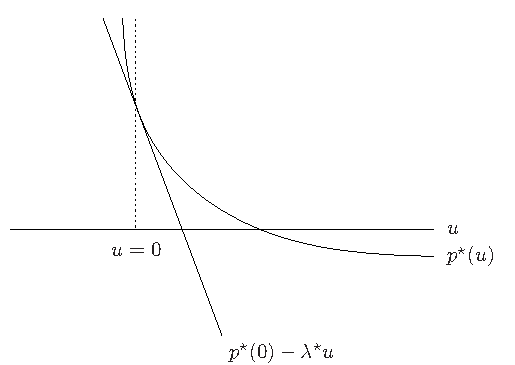
\includegraphics[width=.65\linewidth]{figures/ch05-fig10.pdf}
\caption*{图5.10\quad 含单个约束 $f_1(x)\le u$ 的凸问题的最优值 $p^\star(u)$ 关于 $u$ 的函数。$u=0$ 时为原未扰动问题；$u<0$ 时约束收紧；$u>0$ 时约束放宽。仿射函数 $p^\star(0)-\lambda^\star u$ 是 $p^\star$ 的下界。}
\end{figure}
\begin{itemize}
\item 若 $\lambda_i^\star$ 很大，并收紧第 $i$ 个约束（即取 $u_i<0$），那么最优值 $p^\star(u,v)$ 保证大幅增加。
\item 若 $\nu_i^\star$ 是很大的正数且取 $v_i<0$，或 $\nu_i^\star$ 是绝对值很大的负数且取 $v_i>0$，那么最优值 $p^\star(u,v)$ 保证大幅增加。
\item 若 $\lambda_i^\star$ 很小，并放宽第 $i$ 个约束（$u_i>0$），那么最优值 $p^\star(u,v)$ 不会下降太多。
\item 若 $\nu_i^\star$ 是很小的正数且 $v_i>0$，或 $\nu_i^\star$ 是绝对值很小的负数且 $v_i<0$，那么最优值 $p^\star(u,v)$ 不会下降太多。
\end{itemize}
不等式（5.57）和上述结论给出扰动后最优值的下界，却不提供上界。因此，关于收紧和放宽约束，这些结果并不对称。例如，设 $\lambda_i^\star$ 很大，并稍微放宽第 $i$ 个约束（即取很小的正 $u_i$），这时（5.57）并无用处；例如，它并不意味着最优值会显著下降。

图5.10用一个仅含一个不等式约束的凸问题说明（5.57）。不等式表示，仿射函数 $p^\star(0)-\lambda^\star u$ 是凸函数 $p^\star$ 的下界。

\subsection{局部灵敏度分析}
现在设 $p^\star(u,v)$ 在 $u=0,v=0$ 处可微。那么，只要强对偶成立，最优对偶变量 $\lambda^\star,\nu^\star$ 就与该点处 $p^\star$ 的梯度相关：

% Source PDF page 266 (printed p. 252)
\begin{equation}
\lambda_i^\star=-\frac{\partial p^\star(0,0)}{\partial u_i},
\qquad
\nu_i^\star=-\frac{\partial p^\star(0,0)}{\partial v_i}.\tag{5.58}
\end{equation}
图5.10的例子说明了这一性质：$-\lambda^\star$ 是 $p^\star$ 在 $u=0$ 附近的斜率。

因此，若 $p^\star(u,v)$ 在 $u=0,v=0$ 处可微且强对偶成立，最优拉格朗日乘子恰好给出最优值关于约束扰动的局部灵敏度。与不可微情形不同，这一解释是对称的：将第 $i$ 个不等式约束稍微收紧（取很小的负 $u_i$），使 $p^\star$ 大约增加 $-\lambda_i^\star u_i$；稍微放宽第 $i$ 个约束（取很小的正 $u_i$），使 $p^\star$ 大约下降 $\lambda_i^\star u_i$。

为证明（5.58），设 $p^\star(u,v)$ 可微且强对偶成立。对扰动 $u=te_i,v=0$，其中 $e_i$ 为第 $i$ 个单位向量，有
\[
\lim_{t\to0}\frac{p^\star(te_i,0)-p^\star}{t}
=\frac{\partial p^\star(0,0)}{\partial u_i}.
\]
由（5.57），当 $t>0$ 时，
\[
\frac{p^\star(te_i,0)-p^\star}{t}\ge-\lambda_i^\star,
\]
而 $t<0$ 时不等式方向相反。取 $t>0$ 且 $t\to0$，得到
\[
\frac{\partial p^\star(0,0)}{\partial u_i}\ge-\lambda_i^\star.
\]
从 $t<0$ 一侧取极限，则得到反方向不等式，因此
\[
\frac{\partial p^\star(0,0)}{\partial u_i}=-\lambda_i^\star.
\]
用同样方法可得
\[
\frac{\partial p^\star(0,0)}{\partial v_i}=-\nu_i^\star.
\]

局部灵敏度结果（5.58）定量衡量一个约束在最优点 $x^\star$ 处的活跃程度。若 $f_i(x^\star)<0$，约束不活跃，可将它稍微收紧或放宽，而不影响最优值。由互补松弛，相应最优拉格朗日乘子必为零。再设 $f_i(x^\star)=0$，即第 $i$ 个约束在最优点处活跃。第 $i$ 个最优拉格朗日乘子给出活跃程度：若 $\lambda_i^\star$ 小，表示稍微放宽或收紧约束对最优值影响不大；若 $\lambda_i^\star$ 大，表示稍微放宽或收紧约束会对最优值产生很大影响。

% Source PDF page 267 (printed p. 253)
\subsubsection*{影子价格解释}
还可以用经济学对结果（5.58）作一个简单的几何解释。为简便，考虑不含等式约束、满足Slater条件的凸问题。变量 $x\in\R^m$ 决定企业的运营方式，目标 $f_0$ 为成本，即 $-f_0$ 为利润。每个约束 $f_i(x)\le0$ 代表对某种资源的限制，例如劳动力、钢材或仓储空间。扰动最优成本函数的相反数 $-p^\star(u)$，告诉我们企业得到更多或更少各类资源时，利润会增加或减少多少。如果它在 $u=0$ 附近可微，则
\[
\lambda_i^\star=-\frac{\partial p^\star(0)}{\partial u_i}.
\]
换言之，$\lambda_i^\star$ 近似表示资源 $i$ 的可用量略微增加时，企业能多获得多少利润。

因此，若允许企业买卖资源 $i$，$\lambda_i^\star$ 就是它的自然价格或均衡价格。例如，若企业可以买卖资源 $i$，价格低于 $\lambda_i^\star$，企业当然会买入一些资源，借此改变运营方式，所增加的利润会超过购买资源的成本。反之，若价格高于 $\lambda_i^\star$，企业会卖出部分已分配资源，并获得净收益，因为出售资源的收入高于资源可用量下降造成的利润损失。

\section{例子}
本节通过例子说明，对问题作简单的等价改写，可能得到非常不同的对偶问题。考虑以下改写方式：
\begin{itemize}
\item 引入新变量及相应等式约束。
\item 用原目标的递增函数替代目标。
\item 使显式约束隐含化，即将它们并入目标函数的定义域。
\end{itemize}

\subsection{引入新变量和等式约束}
考虑无约束问题
\begin{equation}
\text{最小化}\quad f_0(Ax+b).\tag{5.59}
\end{equation}
它的拉格朗日对偶函数为常数 $p^\star$。因此，虽然强对偶成立，即 $p^\star=d^\star$，但拉格朗日对偶既无用，也不令人感兴趣。

% Source PDF page 268 (printed p. 254)
现在把（5.59）改写为
\begin{equation}
\begin{array}{ll}\text{最小化}&f_0(y)\\
\text{约束为}&Ax+b=y.\end{array}\tag{5.60}
\end{equation}
这里引入新变量 $y$ 和新等式约束 $Ax+b=y$。问题（5.59）与（5.60）显然等价。

改写后问题的拉格朗日函数为
\[
L(x,y,\nu)=f_0(y)+\nu^\T(Ax+b-y).
\]
对 $x,y$ 最小化 $L$，即可求对偶函数。先对 $x$ 最小化，得到：除非 $A^\T\nu=0$，否则 $g(\nu)=-\infty$；当等式成立时，剩下
\[
g(\nu)=b^\T\nu+\inf_y(f_0(y)-\nu^\T y)=b^\T\nu-f_0^*(\nu),
\]
其中 $f_0^*$ 是 $f_0$ 的共轭。因此（5.60）的对偶可写为
\begin{equation}
\begin{array}{ll}\text{最大化}&b^\T\nu-f_0^*(\nu)\\
\text{约束为}&A^\T\nu=0.\end{array}\tag{5.61}
\end{equation}
所以，改写后问题（5.60）的对偶比原问题（5.59）的对偶有用得多。

\begin{origexample}{5.5}
\emph{无约束几何规划。}考虑无约束几何规划
\[
\text{最小化}\quad\log\left(\sum_{i=1}^m\exp(a_i^\T x+b_i)\right).
\]
首先引入新变量和等式约束，将其改写为
\[
\begin{array}{ll}\text{最小化}&f_0(y)=\log\left(\sum_{i=1}^m\exp y_i\right)\\
\text{约束为}&Ax+b=y,\end{array}
\]
其中 $a_i^\T$ 为 $A$ 的各行。指数和的对数函数的共轭为
\[
f_0^*(\nu)=\begin{cases}
\sum_{i=1}^m\nu_i\log\nu_i&\nu\succeq0,\ \one^\T\nu=1,\\
\infty&\text{其他情形}
\end{cases}
\]
（第93页例3.25），所以改写后问题的对偶可写为
\begin{equation}
\begin{array}{ll}\text{最大化}&b^\T\nu-\sum_{i=1}^m\nu_i\log\nu_i\\
\text{约束为}&\one^\T\nu=1\\&A^\T\nu=0\\&\nu\succeq0,\end{array}\tag{5.62}
\end{equation}
这是一个熵最大化问题。
\end{origexample}

\begin{origexample}{5.6}
\emph{范数逼近问题。}考虑无约束范数逼近问题
\begin{equation}
\text{最小化}\quad\norm{Ax-b},\tag{5.63}
\end{equation}
其中 $\norm{\cdot}$ 为任意范数。这里拉格朗日对偶函数同样为常数，等于（5.63）的最优值，因此没有用处。
